% !TEX program = lualatex
\documentclass[12pt,a4paper]{article}
\usepackage{fontspec}
\setmonofont{Latin Modern Mono}
\usepackage{xcolor}
\usepackage{listings}
\usepackage{geometry}
\usepackage{fancyhdr}
\usepackage{hyperref}
\usepackage{graphicx}
\geometry{margin=1in}
\usepackage{multicol}

% -------------------------------
% Header and Footer Configuration
% -------------------------------
\pagestyle{fancy}
\fancyhf{}
\lhead{Lab 3: Introduction to DDL and DML Operations}
\rhead{CSE 4308: DBMS Lab}

% Centered footer with page number
\cfoot{\thepage}
% Ensure header/footer width matches text block
\setlength{\headwidth}{\textwidth}

% -------------------------------
% Code Listing Style
% -------------------------------
\definecolor{codegreen}{rgb}{0,0.6,0}
\definecolor{codegray}{rgb}{0.5,0.5,0.5}
\definecolor{codepurple}{rgb}{0.58,0,0.82}
\definecolor{backcolour}{rgb}{0.95,0.95,0.92}

\lstdefinestyle{mystyle}{
    backgroundcolor=\color{backcolour},
    commentstyle=\color{codegreen},
    keywordstyle=\color{magenta},
    numberstyle=\tiny\color{codegray},
    stringstyle=\color{codepurple},
    basicstyle=\ttfamily\footnotesize,
    breaklines=true,
    captionpos=b,
    keepspaces=true,
    numbers=none,
    numbersep=5pt,
    tabsize=2,
    frame=single,
    columns=fullflexible,
    showspaces=false,
    showstringspaces=false,
    showtabs=false
}

\lstset{style=mystyle}

% Images: found next to this file (local compile_labs.sh) or via the
% lab folder when compiled from the project root (Overleaf).
\graphicspath{{lab_03_ddl_dml/}{../}}

\begin{document}

% --------------------------------------------------------------
% TITLE PAGE
% --------------------------------------------------------------
\begin{titlepage}
    \centering
    \vspace*{2\baselineskip}

    \rule{14cm}{2pt}\vspace*{-0.8\baselineskip}\vspace*{1.5pt}
    \rule{14cm}{0.5pt}\vspace{2\baselineskip}

    {\Huge\bfseries\scshape Lab 3\par}
    \vspace{3mm}
    {\Large Introduction to DDL and DML Operations\par}
    \vspace{2mm}
    {\large Group 1B\par}
    \vspace{3mm}

    \rule{14cm}{0.5pt}\vspace*{-0.7\baselineskip}\vspace{2.5pt}
    \rule{14cm}{2pt}

    \vspace{2\baselineskip}

    {\Large\bfseries CSE 4308\par}
    \vspace{1\baselineskip}
    {\large DATABASE MANAGEMENT SYSTEMS LAB\par}

    \vfill
    {\normalsize Prepared by:\\ Samnun Azfar, Jr. Lecturer, CSE\\ Samia Nawsheen, Jr. Lecturer, CSE\par}
    {\normalsize Academic Year: AY25-26\par}
\end{titlepage}

\newpage

% ==============================================================
\section{Table Management (DDL)}

\subsection{Creating a Table}
Creating a table defines the structure of your data. You must define columns, data types, and constraints.

\textbf{General Syntax:}
\begin{lstlisting}
CREATE TABLE table_name
(
    attribute1 datatype [ NULL | NOT NULL | UNIQUE ],
    attribute2 datatype [ NULL | NOT NULL | UNIQUE ],
    ...
);
\end{lstlisting}

\subsubsection{Common PostgreSQL Data Types}
\begin{itemize}
    \item \texttt{INT}: Standard whole numbers. \textit{Warning: Removes leading zeros (001 becomes 1).}
    \item \texttt{VARCHAR(n)}: Variable-length string. \textbf{Use this for IDs with leading zeros} (e.g., Zip Codes, Student IDs like \texttt{'00128'}).
    \item \texttt{CHAR(n)}: Fixed-length string. Pads with spaces if input is short.
    \item \texttt{SERIAL}: Auto-incrementing integer (1, 2, 3...). Perfect for internal IDs.
    \item \texttt{NUMERIC(p,s)}: Exact decimals (e.g., Currency).
    \item \texttt{DATE}: Calendar dates.
\end{itemize}

\subsubsection{Example: Constraints}
Constraints protect data quality.
\begin{lstlisting}
CREATE TABLE PRODUCT
(
    PID SERIAL PRIMARY KEY,         -- Unique, Auto-increment
    PNAME VARCHAR(50) NOT NULL,     -- Cannot be empty
    PRICE INT,
    CONSTRAINT PRICE_CHECK CHECK (PRICE >= 0) -- No negative prices
);
\end{lstlisting}

\subsection{Dropping Tables}
\begin{lstlisting}
DROP TABLE table_name;
\end{lstlisting}

\textbf{The Cascade Option:}
If other objects depend on this table, use \texttt{CASCADE} to force deletion.
\begin{lstlisting}
DROP TABLE PRODUCT CASCADE;
\end{lstlisting}

\subsection{Altering Tables}
Modify structure without deleting data.

\begin{lstlisting}
-- 1. Add a new column
ALTER TABLE PRODUCT ADD COLUMN STOCK INT;

-- 2. Remove a column
ALTER TABLE PRODUCT DROP COLUMN STOCK;

-- 3. Change data type
ALTER TABLE PRODUCT ALTER COLUMN PRICE TYPE NUMERIC(10,2);

-- 4. Rename column
ALTER TABLE PRODUCT RENAME COLUMN PNAME TO PRODUCT_NAME;
\end{lstlisting}

\section{Data Manipulation (DML)}

\subsection{Inserting Records}
\textbf{Named Notation (Recommended):}
Specifying columns is safer than relying on column order.
\begin{lstlisting}
INSERT INTO PRODUCT(PID, PNAME, PRICE) VALUES (DEFAULT, 'Pen', 15);
\end{lstlisting}

\subsection{Updating Data}
\textbf{Warning:} Always use a \texttt{WHERE} clause, otherwise all rows are updated.
\begin{lstlisting}
UPDATE PRODUCT
SET PRICE = 250
WHERE PID = 1;
\end{lstlisting}

\subsection{Deleting Data}
\textbf{Warning:} Without a \texttt{WHERE} clause, the table becomes empty.
\begin{lstlisting}
DELETE FROM PRODUCT
WHERE PRICE = 0;
\end{lstlisting}

\subsection{Retrieval (SELECT) and Filtering}
The core of SQL is querying data.

\textbf{Basic Filtering:}
\begin{lstlisting}
SELECT * FROM PRODUCT WHERE PRICE > 50;
\end{lstlisting}

\subsubsection{Logical Operators (AND, OR)}
To answer complex questions, we combine conditions.

\textbf{1. AND Operator:}
Both conditions must be true.
\begin{lstlisting}
-- Find products that are expensive AND in a specific category
SELECT * FROM PRODUCT 
WHERE PRICE > 100 AND CATEGORY = 'Electronics';
\end{lstlisting}

\textbf{2. OR Operator:}
At least one condition must be true.
\begin{lstlisting}
-- Find products that are either Blue OR Red
SELECT * FROM PRODUCT 
WHERE COLOR = 'Blue' OR COLOR = 'Red';
\end{lstlisting}
\newpage
\section*{Lab Workflow}

\textit{Repeat this subsection for every single lab.}

\begin{enumerate}
\item Connect to the internet by running nmtui in terminal, add a dsl connection, then go back and activate that dsl connection. Make sure that your net id is not being used in any other pc or router, if you face any issue, use any other net id from your friends which is not being used.

\item Download all the files posted in the google classroom.

\item Disconnect from the \textbf{dsl} connection via nmtui, connect to the ethernet/wired connection via nmtui. If no such connection exists, create an \textbf{ethernet} connection  and then activate.

    \item \textbf{Create Your Role and Database}

Inside the PostgreSQL shell, create your own role (user) and database.

1. In the Linux terminal:
\begin{lstlisting}[language=bash]
psql
\end{lstlisting}

Expected prompt:
\begin{lstlisting}
cse=#
\end{lstlisting}

2. Create Your Role and Database

Copy and run the following commands inside PostgreSQL:
\begin{lstlisting}[language=SQL]
-- 1. Terminate existing database connections
SELECT pg_terminate_backend(pid)
FROM pg_stat_activity
WHERE datname = 'cse4308_12345'
  AND pid <> pg_backend_pid();

-- 2. Remove existing database
DROP DATABASE IF EXISTS cse4308_12345;

-- 3. Remove existing role
DROP ROLE IF EXISTS student_12345;

-- 4. Create role
CREATE ROLE student_12345 LOGIN;

-- 5. Set password
ALTER ROLE student_12345
WITH PASSWORD 'student12345';

-- 6. Create database
CREATE DATABASE cse4308_12345
OWNER student_12345;

-- 7. Grant privileges
GRANT ALL PRIVILEGES
ON DATABASE cse4308_12345
TO student_12345;
\end{lstlisting}

3. Exit PostgreSQL:

   \begin{lstlisting}[language=SQL]
   \q
   \end{lstlisting}

\item \textbf{Connect Using Your Newly Created User}

1. Connect to Your Database:

   Use the following command to log in as the \texttt{student\_12345} user:

   \begin{lstlisting}[language=SQL]
   psql -h localhost -U student_12345 -d cse4308_12345
   \end{lstlisting}

2. Verify the Connection:

   Verify that you are connected to the correct database with the following command:

   \begin{lstlisting}[language=SQL]
   \conninfo
   \end{lstlisting}

   Expected output:

   \begin{lstlisting}
   You are connected to database "cse4308_12345" as user "student_12345".
   \end{lstlisting}

3. Exit PostgreSQL:

   \begin{lstlisting}[language=SQL]
   \q
   \end{lstlisting}

\item \textbf{Load the Lab SQL File (MUST be run outside psql)}

Load the SQL file that sets up the tables and inserts initial data.

1. Load the SQL File:

   Run the following command to load the lab SQL file:

   \begin{lstlisting}[language=SQL]
   psql -h localhost -U student_12345 -d cse4308_12345 -f /home/cse/Downloads/lab_03_1b_setup.sql
   \end{lstlisting}

   This will:
   - Drop old tables (if they exist).
   - Create new tables.
   - Insert initial rows of data.

\item \textbf{Reconnect and Verify Tables}

After loading the SQL file, reconnect to PostgreSQL to verify that the tables have been created.

1. Reconnect to Your Database:

   \begin{lstlisting}[language=SQL]
   psql -h localhost -U student_12345 -d cse4308_12345
   \end{lstlisting}

2. Check Tables:

   Verify the tables have been created by listing them:

   \begin{lstlisting}[language=SQL]
   \dt
   \end{lstlisting}

3. View Table Data:

   Verify the data by running the following SQL queries:

   \begin{lstlisting}[language=SQL]
   SELECT * FROM <table_name>;
   \end{lstlisting}

\item Open a text editor and save it in the appropriate submission name format \\ \texttt{fullid\_CSE4308\_L3\_T1.sql}. You will use this text editor to write your solutions, make sure to save it after writing each solution. The structure of this file will be:
\begin{lstlisting}[language=SQL]
-- Task 1
INSERT INTO students (student_id, name, major, gpa)
VALUES (104, 'David', 'ME', 3.60);
--Task 2
SELECT name, gpa FROM students WHERE major = 'CSE';
\end{lstlisting}
\end{enumerate}
\newpage
\section{Lab Task}
\noindent % Prevents paragraph indentation so the columns fit
\begin{minipage}[t]{0.48\textwidth}
    \vspace{0pt} % A trick to force top alignment for lists
    The \texttt{EMPLOYEE} table:
    \begin{itemize}
        \item \texttt{ID} (Primary Key)
        \item \texttt{NAME} (Must not be NULL)
        \item \texttt{DEPT\_NAME}
        \item \texttt{SALARY} 
    \end{itemize}
\end{minipage}%
\hfill % This adds flexible space between the two columns
\begin{minipage}[t]{0.48\textwidth}
    \vspace{0pt} % A trick to force top alignment
    \centering
    % Do NOT use \begin{figure} here
    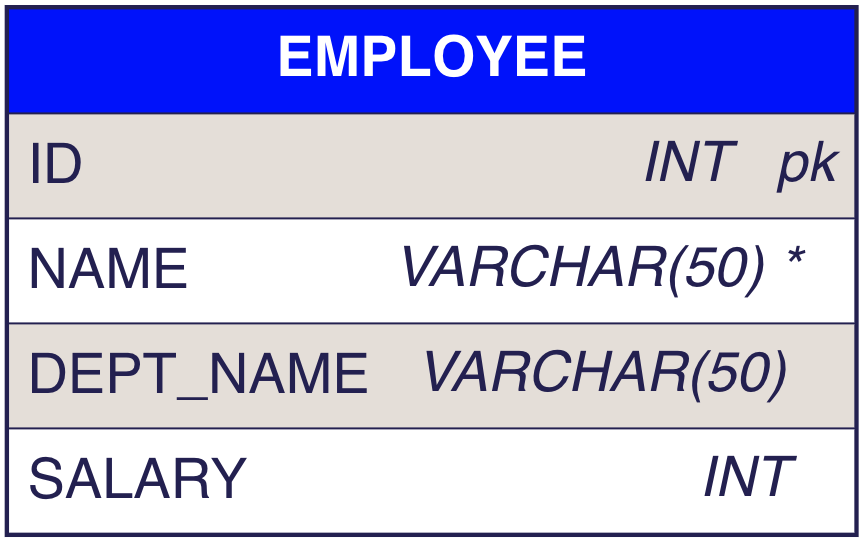
\includegraphics[width=0.6\linewidth]{lab_03_figure.png}
    % If you need a caption, use \captionof{figure}{Your caption} (requires caption package)
\end{minipage}
    
    \begin{table}[h!]\centering
    \begin{tabular}{|c|l|l|c|}
        \hline
        \textbf{ID} & \textbf{NAME} & \textbf{DEPT\_NAME} & \textbf{SALARY} \\ \hline
        00128 & Zhang & Machinery & 1060 \\
        12345 & Shankar & Finance & 3200 \\
        19991 & Brandt & Finance & 80000 \\
        23121 & Chavez & Sales & 11000 \\
        44553 & Peltier & Machinery & 5750 \\
        45678 & Levy & Sales & 460 \\
        54321 & Williams & Finance & 45000 \\
        55739 & Sanchez & Research & 38100 \\ 
        70557 & Snow & Machinery & 0 \\
        76543 & Brown & Research & 5800 \\
        76653 & Aoi & Research & 0 \\
        98765 & Bourikas & Sales & 9000 \\
        98988 & Tanaka & Machinery & 1200 \\ \hline
    \end{tabular}
    \end{table}

\noindent Create the \texttt{EMPLOYEE} table, then insert the data as shown in the \texttt{EMPLOYEE} table by running \texttt{lab\_03\_1b\_setup.sql}. Then perform the following queries on the \texttt{EMPLOYEE} table:
\begin{enumerate}
    \item Display all records of the \texttt{EMPLOYEE} table.
    \item Find the names of employees from Finance department who earn more than 7,000.
    % \item Show the ID and name of employees earning between 10,000 and 50,000.
    \item Find the names of employees working in either Sales or Research.
    % \item Show the names of the departments containing employees named `Shankar' or `Sanchez'.
    \item Delete employees who are working without salary (\texttt{SALARY = 0}).
    \item Drop the \texttt{EMPLOYEE} table.

\end{enumerate}

\end{document}